\section{Swaption Pricing} \label{swaption_price_sec}
Now we hav seen that the implied volatility can change over various tenors. 
Therefore it is important to be aware of how the volatility affect the market.
And thereby which asset there maybe will perform in different situations i the market,
due to high or low volatility, inflation and other factor the can influence the market.
When it comes to swaption and other asset the volatility also has
a remarkable determination of the price of the asset. 
\\\\
In the Section \ref{invest_sabr} we learned how the different parameters in the 
SABR model affects the implied volatility in swaption. 
Where in Section \ref{est_parm_sabr} we estimated the parameters in the SABR model. 
From these Sections we saw some clear coincidence between the level of a given parameter
and the effect on the implied volatility. 
This implied volatility determine from the SABR model, is then used to price swaption using the 
Black-Scholes model. 
Therefor we have computed the prices for swaption with a fixed expiry at 10 years and for various tenors. 
The price are ATM, which means that, F, the forward rate is equal to, K, 
the strike (the rate of the underlying asset). 
\\\\
Below in \autoref{tab:swaption_price_atm} the calculated prices for the various swaption 
using the describe method is listed. 
The prices are ATM prices for a fixed tenor at 10 yeas and for various tenors. 
To illustrated the development of the price over the different tenors, 
the swaption price is despited below in  \autoref{fig:swaption_price_atm}.
\begin{table}[H]
  \centering
  \begin{tabular}{ccccccccccc}
    \toprule
    \textbf{ Tenor} & 1Y & 2Y & 3Y & 5Y & 7Y & 10Y & 12Y & 15Y & 20Y & 30Y \\
    \midrule
    \textbf{ Swaption price }&0.1334 & 0.1351 & 0.1360 &0.1358  &0.1336  &0.1289
    &0.1254& 0.1205 & 0.1143 & 0.1062 \\
    \bottomrule
  \end{tabular}
  \caption{ATM swaption price in basis point for a 10 years fixed expiry and various tenors.
  Data source  \\ Citi Velocity 21.02.2024}
  \label{tab:swaption_price_atm}
\end{table}
\noindent
\autoref{fig:swaption_price_atm} shows a decreasing tends in swaptions prices as the tenor increases,
starting off relatively flat in the shorter durations tenors (1 to 5 years) and then 
descending more steeply from around the 5 year tenor. 
The pattern in the graph indicates that the longer the duration of the swaptions tenor, 
the lower the cost to enter into one. A swaption is essentially an option that grants the 
holder the right, but not the obligation, to initiate a swap agreement with specific terms at a future date. 
The graph shows that swaption prices are relatively stable for shorter tenors and begin to 
decrease more noticeably for durations extending beyond 5 years. 
This flattening in the initial period could be due to more predictable or stable interest 
rate expectations in the near term. Conversely, the significant price drop for longer 
tenors might suggest greater uncertainty or a reduced interest in securing rate locks for extended periods.
\begin{figure}[H]
    \centering
    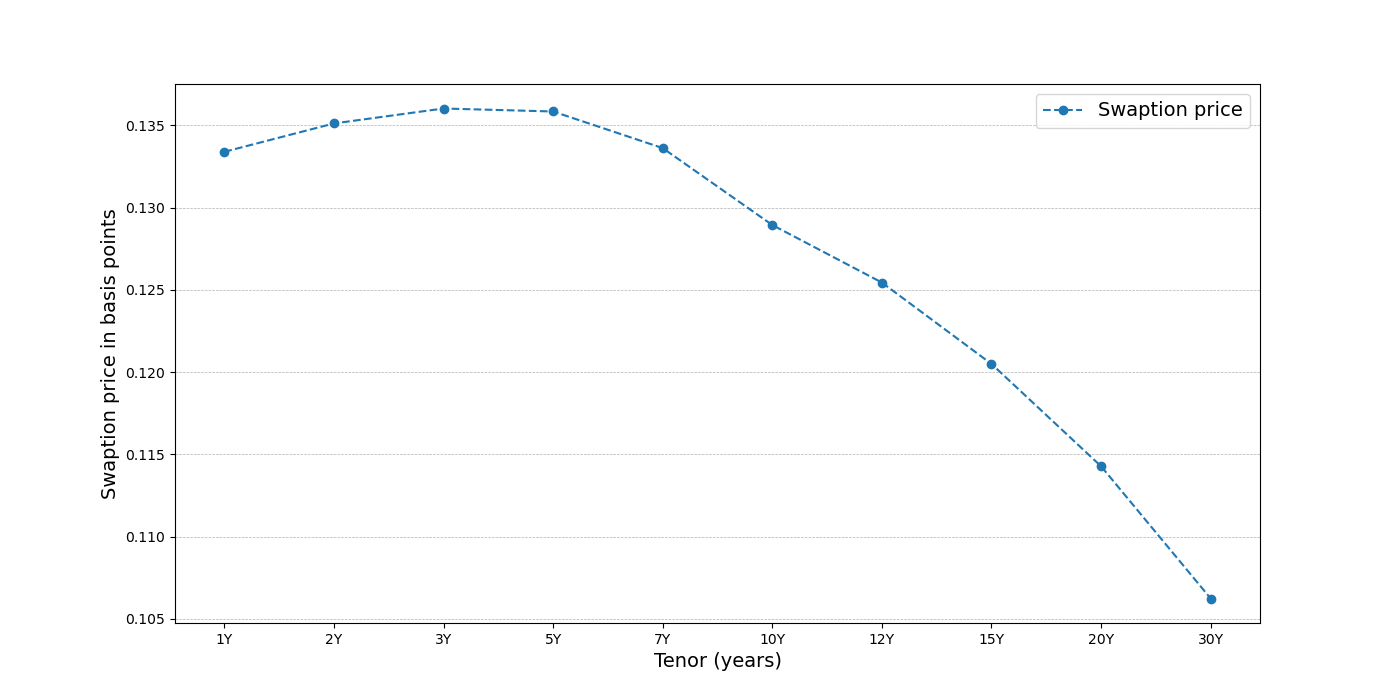
\includegraphics[scale = 0.5]{/Users/nannaingemannohrt/Desktop/master_thesis/main/plots/swaption_price_atm.png}
    \caption{ATM swaption price in basis point for a 10 years fixed expiry and various tenors.
    Data source  \\ Citi Velocity 21.02.2024}
    \label{fig:swaption_price_atm}
\end{figure}
\noindent
So in other words \autoref{fig:swaption_price_atm}  could indicate that swaptions with a lower is less
volatile than longer duration tenor swaption. This could be exampled by that in finance we will 
expected short terms interest rate to behave like the short rate in the Vasicek model for example. 
We in the Vasicek model we learned that the short rate tend to a mean reverting level. 
So there will not be expected larger fluctuations on short term, but we don't know how the market is in 
30 years. But if we compare the shape of the calculated swaptions price in \autoref{fig:swaption_price_atm} 
to shape of the forward \autoref{fig:forward_plot}. We see that the same tendency in the slope 
is represented. Hence the market expectations the that the forward is lower for longer duration tenor, 
than for short duration tenor. 
\\\\
But as mentioned there are other factor there affect the price of a swaption than the level of the forward. 
Also the other parameters in the SABR model also affect the swaption price indirect, 
since the parameter effect the implied volatility. 
So as promise Chapter \ref{risk_mang} we will look into the sensitivities in the SABR model.
